\documentclass[12t,letterpaper]{article}

\newenvironment{proof}{\noindent{\bf Proof:}}{\qed\bigskip}

\newtheorem{theorem}{Theorem}
\newtheorem{corollary}{Corollary}
\newtheorem{lemma}{Lemma} 
\newtheorem{claim}{Claim}
\newtheorem{fact}{Fact}
\newtheorem{definition}{Definition}
\newtheorem{assumption}{Assumption}
\newtheorem{observation}{Observation}
\newtheorem{example}{Example}
\newcommand{\qed}{\rule{7pt}{7pt}}

\newcommand{\assignment}[4]{
\thispagestyle{plain} 
\newpage
\setcounter{page}{1}
\noindent
\begin{center}
\framebox{ \vbox{ \hbox to 6.28in
{\bf CS446: Machine Learning \hfill #1}
\vspace{4mm}
\hbox to 6.28in
{\hspace{2.5in}\large\mbox{#2}}
\vspace{4mm}
\hbox to 6.28in
{{\it Handed Out: #3 \hfill Due: #4}}
}}
\end{center}
}

\newcommand{\solution}[3]{
\thispagestyle{plain} 
\newpage
\setcounter{page}{1}
\noindent
\begin{center}
\framebox{ \vbox{ \hbox to 6.28in
{\bf CS 374 \hfill #3}
\vspace{4mm}
\hbox to 6.28in
{\hspace{2.5in}\large\mbox{#2}}
\vspace{4mm}
\hbox to 6.28in
{#1 \hfill}
}}
\end{center}
\markright{#1}
}

\newenvironment{algorithm}
{\begin{center}
\begin{tabular}{|l|}
\hline
\begin{minipage}{1in}
\begin{tabbing}
\quad\=\qquad\=\qquad\=\qquad\=\qquad\=\qquad\=\qquad\=\kill}
{\end{tabbing}
\end{minipage} \\
\hline
\end{tabular}
\end{center}}

\def\Comment#1{\textsf{\textsl{$\langle\!\langle$#1\/$\rangle\!\rangle$}}}


\usepackage{amsmath, verbatim, tikz, float}

\usetikzlibrary{arrows,automata}

\oddsidemargin 0in
\evensidemargin 0in
\textwidth 6.5in
\topmargin -0.5in
\textheight 9.0in
\newcommand{\norm}[1]{\left\lVert #1 \right\rVert}
\begin{document}

\solution{Nikhil Unni (nunni2)}{Homework 2}{Spring 2015}
\pagestyle{myheadings}

\begin{enumerate}
  \setcounter{enumi}{2}
\item
  \begin{enumerate}
    \item 
      The two languages $L(M)$ and $L(\overline{M})$ are complements of one another. Because we switch the non-accepting and accepting states, we are now accepting all other possible strings in the language $\Sigma^*$, and excluding all in $L(M)$. In other words, $L(\overline{M}) = \overline{L(M)}$.
    \item
      $L(\overline{M})$ does not necessarily hold a set relationship\footnote{https://piazza.com/class/i4mrvddxr0h3sd?cid=368} with L(M). For example, looking back at the NFA from 1b.i : 
      \begin{figure}[H]
      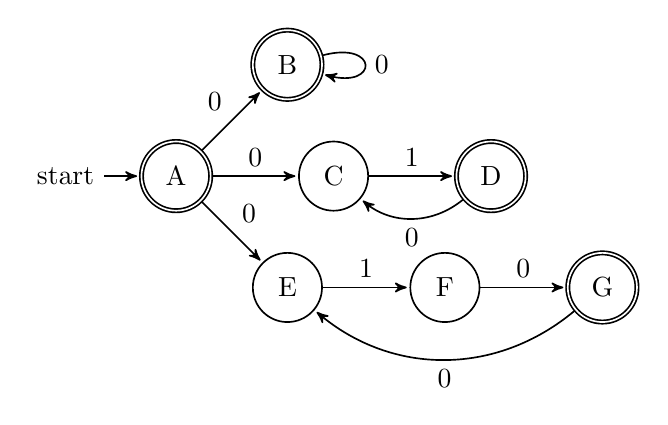
\begin{tikzpicture}[->,>=stealth',shorten >=1pt,auto,node distance=2.0cm, semithick]
        \tikzstyle{every state}=[fill=none,draw=black,text=black]
        \node[initial,state,accepting] (A)                    {A};

        \node[state,accepting]         (B) [above right of=A] {B};

        \node[state]                   (C) [right of=A]       {C};
        \node[state,accepting]         (D) [right of=C]       {D};

        \node[state]                   (E) [below right of=A] {E};
        \node[state]                   (F) [right of=E]       {F};
        \node[state,accepting]         (G) [right of=F]       {G};

        \path (A) edge                node {0} (B)
                  edge                node {0} (C)
                  edge                node {0} (E)
              (B) edge [loop right]   node {0} (B)
              (C) edge                node {1} (D)
              (D) edge [bend left=40] node {0} (C)
              (E) edge                node {1} (F)
              (F) edge                node {0} (G)
              (G) edge [bend left=40] node {0} (E);
      \end{tikzpicture}
      \end{figure}
      Switching, we get:
      \begin{figure}[H]
      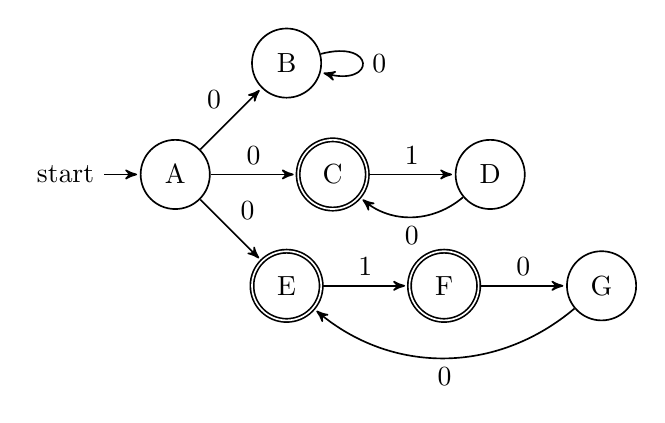
\begin{tikzpicture}[->,>=stealth',shorten >=1pt,auto,node distance=2.0cm, semithick]
        \tikzstyle{every state}=[fill=none,draw=black,text=black]
        \node[initial,state]   (A)                    {A};

        \node[state]           (B) [above right of=A] {B};

        \node[state,accepting] (C) [right of=A]       {C};
        \node[state]           (D) [right of=C]       {D};

        \node[state,accepting] (E) [below right of=A] {E};
        \node[state,accepting] (F) [right of=E]       {F};
        \node[state]           (G) [right of=F]       {G};

        \path (A) edge                node {0} (B)
                  edge                node {0} (C)
                  edge                node {0} (E)
              (B) edge [loop right]   node {0} (B)
              (C) edge                node {1} (D)
              (D) edge [bend left=40] node {0} (C)
              (E) edge                node {1} (F)
              (F) edge                node {0} (G)
              (G) edge [bend left=40] node {0} (E);
      \end{tikzpicture}
      \end{figure}
      ``01010'' is accepted by both, so $L(\overline{M})$ and $\overline{L(M)}$ cannot be unequal. ``0'' is in $L(\overline{M})$, but not in $\overline{L(M)}$, and ``1'' is in $\overline{L(M)}$, but not $L(\overline{M})$, so one is not necessarily a subset of the other. Since neither is the subset of the other, we know the two cannot be equal. So there are no conclusions we can draw about the relationship of the two sets for any arbitrary NFA.\\

      \item
        Let's call this new NFA, N (similar to the notation from the third problem). Then our NFA is defined as:
        $$Q^N = (2^Q, Q)$$
        $$\Sigma^N = \Sigma$$
        $$\delta^N((q,r), a) = ( (\cup_{p \in q}\delta(p,a) \text{ for all } q' \subseteq Q \text { and } a \in \Sigma), \delta(r) )$$
        $$q_0^N = (\{q_0\}, q_0)$$
        $$F^N = ( \{S \subseteq Q | S \cap F = \emptyset \}, q, q \in F)$$

        It seems a little overkill, but it's just the couplet where the first dimension is the translated-DFA version of M with the final states reversed, representing $\overline{L(M)}$ and the second represents $L(\overline{M})$. The transitions and starting states are all borrowed from the definitions, and the only variation is that now the final states are only when the first dimension is satisfied, and the second dimension is not satisfied (in this case it means that the state is in $F$).


      \item
        Using the same trick we can construct this set difference (sticking to the same dimension order, but changing the conditions in the set of accepting states):
        $$Q^N = (2^Q, Q)$$
        $$\Sigma^N = \Sigma$$
        $$\delta^N((q,r), a) = ( (\cup_{p \in q}\delta(p,a) \text{ for all } q' \subseteq Q \text { and } a \in \Sigma), \delta(r) )$$
        $$q_0^N = (\{q_0\}, q_0)$$
        $$F^N = ( \{S \subseteq Q | S \cap F \neq \emptyset \}, q, q \notin F)$$

  \end{enumerate}
  
\end{enumerate}
\end{document}